\documentclass[a4paper]{tufte-handout}

\title{Le Corbusier - Leben, Denken und Werk}%\thanks{Inspired by Edward~R. Tufte!}}

\author[Lennard Wolf]{Lennard Wolf}

\date{ } % without \date command, current date is supplied

%\geometry{showframe} % display margins for debugging page layout

\usepackage{graphicx} % allow embedded images
  \setkeys{Gin}{width=\linewidth,totalheight=\textheight,keepaspectratio}
  \graphicspath{{graphics/}} % set of paths to search for images
\usepackage{amsmath}  % extended mathematics
\usepackage[ngerman]{babel}
\usepackage{booktabs} % book-quality tables
\usepackage{units}    % non-stacked fractions and better unit spacing
\usepackage{multicol} % multiple column layout facilities
\usepackage{lipsum}   % filler text
\usepackage{fancyvrb} % extended verbatim environments
\usepackage{textcomp}
  \fvset{fontsize=\normalsize}% default font size for fancy-verbatim environments

% Standardize command font styles and environments
\newcommand{\doccmd}[1]{\texttt{\textbackslash#1}}% command name -- adds backslash automatically
\newcommand{\docopt}[1]{\ensuremath{\langle}\textrm{\textit{#1}}\ensuremath{\rangle}}% optional command argument
\newcommand{\docarg}[1]{\textrm{\textit{#1}}}% (required) command argument
\newcommand{\docenv}[1]{\textsf{#1}}% environment name
\newcommand{\docpkg}[1]{\texttt{#1}}% package name
\newcommand{\doccls}[1]{\texttt{#1}}% document class name
\newcommand{\docclsopt}[1]{\texttt{#1}}% document class option name
\newenvironment{docspec}{\begin{quote}\noindent}{\end{quote}}% command specification environment

\begin{document}

\maketitle% this prints the handout title, author, and date


\begin{abstract}
\noindent
\emph{"`Le Corbusier gilt als bedeutendster Architekt des 20. Jahrhunderts. Mit seinen Bauten, seinen B"uchern, aber auch mit seinem Erscheinungsbild -- als \emph{homme machine} mit Fliege und schwarzer Brille -- pr"agte er die Vorstellung, die wir von moderner Architektur, ja von Moderne "uberhaupt haben."'}\footnote{von Vegesack, Alexander (Hrsg.): \emph{Le Corbusier - The Art of Architecture}, Weil am Rhein 2007.}
\end{abstract}

%\printclassoptions

\section{Leben}\label{sec:leben}

\textasteriskcentered ~06. Oktober 1887 (La Chaux-de-Fonds, Schweiz)\\
\noindent \textdagger~27. August 1965 (Roquebrune-Cap-Martin, Frankreich)\\

\newthought{Le Corbusier} (geboren als Charles-\'Edouard Jeanneret-Gris) wuchs wohlhabend und -beh"utet in der Schweiz auf. Seine Mutter war Klavierlehrerin, sein Vater Graveur. Im Alter von 18 Jahren begann er mit Mitstudierenden die Arbeit an der \emph{Villa Fallet} (1905, Chaletstil), zu der Zeit noch stark beeinflusst von der \emph{Arts and Crafts} Bewegung. Er reiste ab dem Alter eines jungen Mannes viel, mit 20 durch ganz Italien, mit 21 nach Wien, M"unchen und Paris. Sp"ater dann u.A. Aufenthalte in Osteuropa, Amerika und Brasilien.

\begin{marginfigure}%
  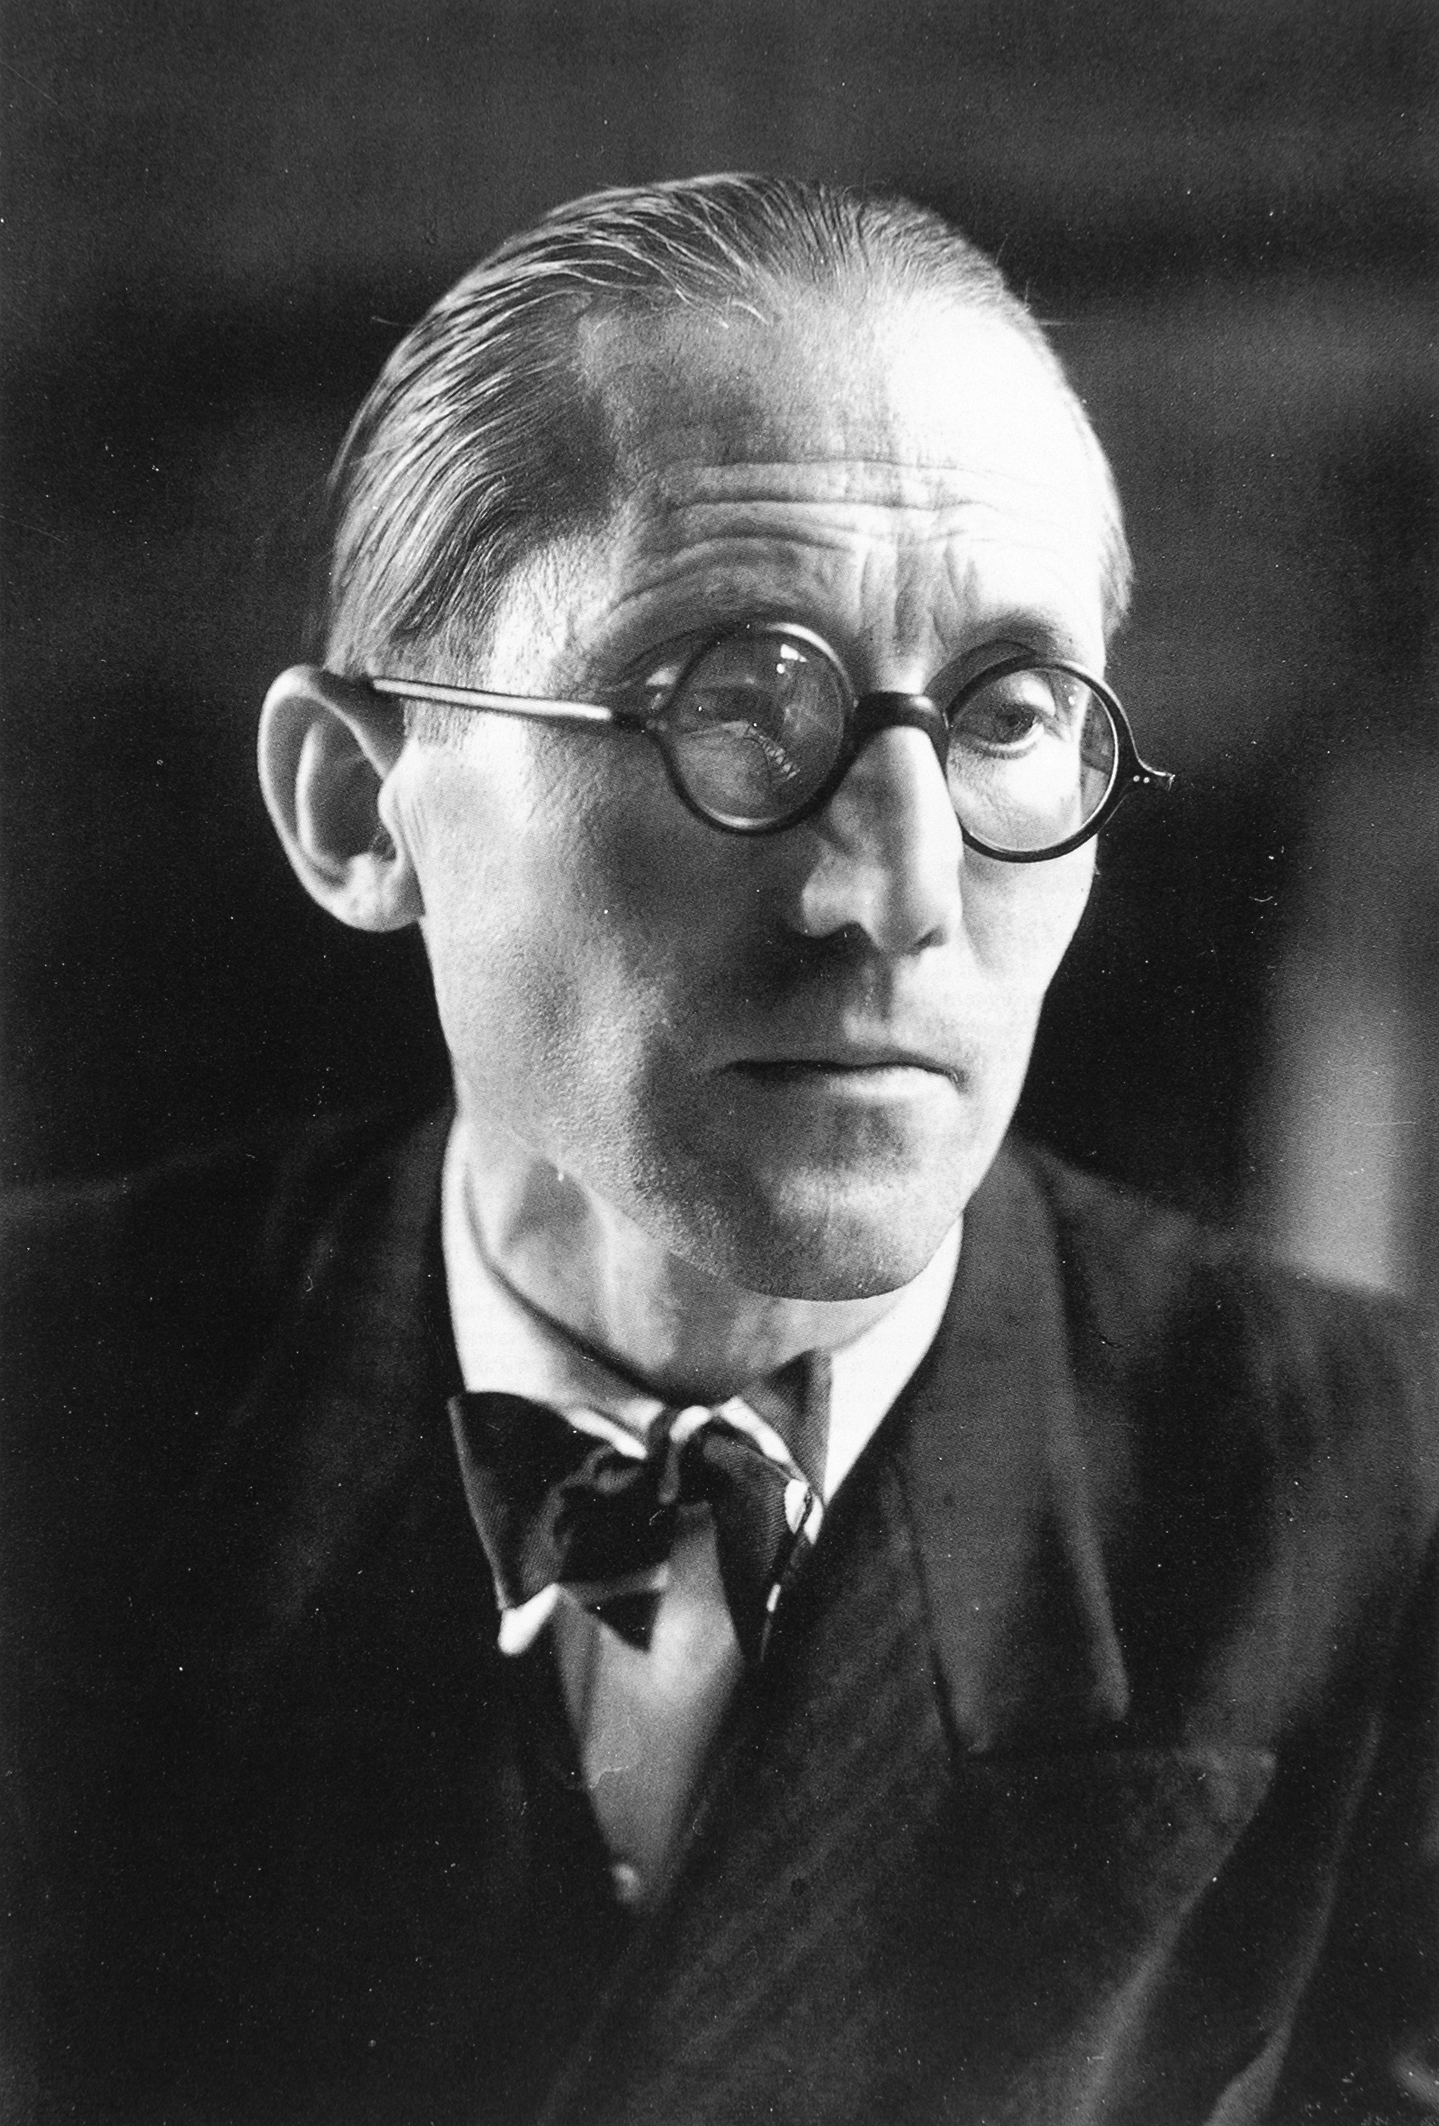
\includegraphics[width=\linewidth]{portrait}
  \caption{Portrait von Le Corbusier}
  \label{fig:portrait}
\end{marginfigure}

\newthought{L'Esprit Nouveau} war die 1920 von ihm mitgegr"undete Zeitschrift, in der Artikel zu ihren Ideen f"ur kontempor"are Kultur ver"offentlicht wurden. In einer ihrer Ausgaben benutze er seinen Pseudonym \emph{Le Corbusier} das erste Mal, als anonymer Architekturkritiker. Dieser Name erlangte sehr schnell gro"se Bekanntheit


\section{Denken}\label{sec:page-layout}

\emph{"`I then recogniced that art -- broader and deeper than anything else -- is the means by which the individual may count completely."'}\footnote{Le Corbusier. \emph{New World of Space.}}

\newthought{Die Mathematik} der Formen faszinierte ihn. Ma"se, Licht, Distanzen, Farben, Linien, Masse: Alles konnte f"ur ihn proportioniert werden. 

\begin{marginfigure}%
  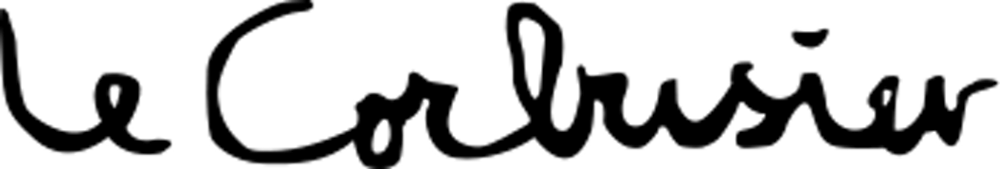
\includegraphics[width=(\linewidth)]{signature.png}
  \caption{Signatur des K"unstlers}
  \label{fig:signature}
\end{marginfigure}


\newthought{Durch die Reisen} entfernte er sich immer weiter von der institutionellen Lehre und n"aherte sich dem autodidaktischen Verstehen von Formen und Materialien, Betrachtung und Bewertung. Das praktische Leben zog ihn an, wie auch das moderne. Er wollte die neuen Materialien seiner Zeit nutzen, um die Menschheit \emph{voran zu bringen}. Entsprechend widmete er sich dem Problem der Obdachlosigkeit durch

\marginnote{\emph{"`For Le Corbusier a work of art [...] organizes and humanizes not merely the space it contains but all the surrounding space, invading brute nature with its own field of force.} -- F.S. Wight im Vorwort von \emph{New World of Space.} }


\newthought{Die f"unf Punkte} zu einer neuen Architektur, vorgestellt in dem gleichnamigen Essay\footnote{Ver"offentlicht in \emph{Vers une architecture.}}, sind \emph{Pfosten}, \emph{Dachg"arten}, \emph{freie Grundrissgestaltung} , \emph{Langfenster} und \emph{freie Fassadengestaltung}.


\section{Werke}\label{sec:werke}

Architektur ist ein zentrales Motiv f"ur das Werk des Le Corbusier, doch geh"oren zu seinem Schaffen auch eine nicht verkennbare Anzahl von Gem"alden, Skulpturen, M"obeln, Zeichnungen und B"uchern.

\subsection{Auswahl}

\begin{figure*}[h]
  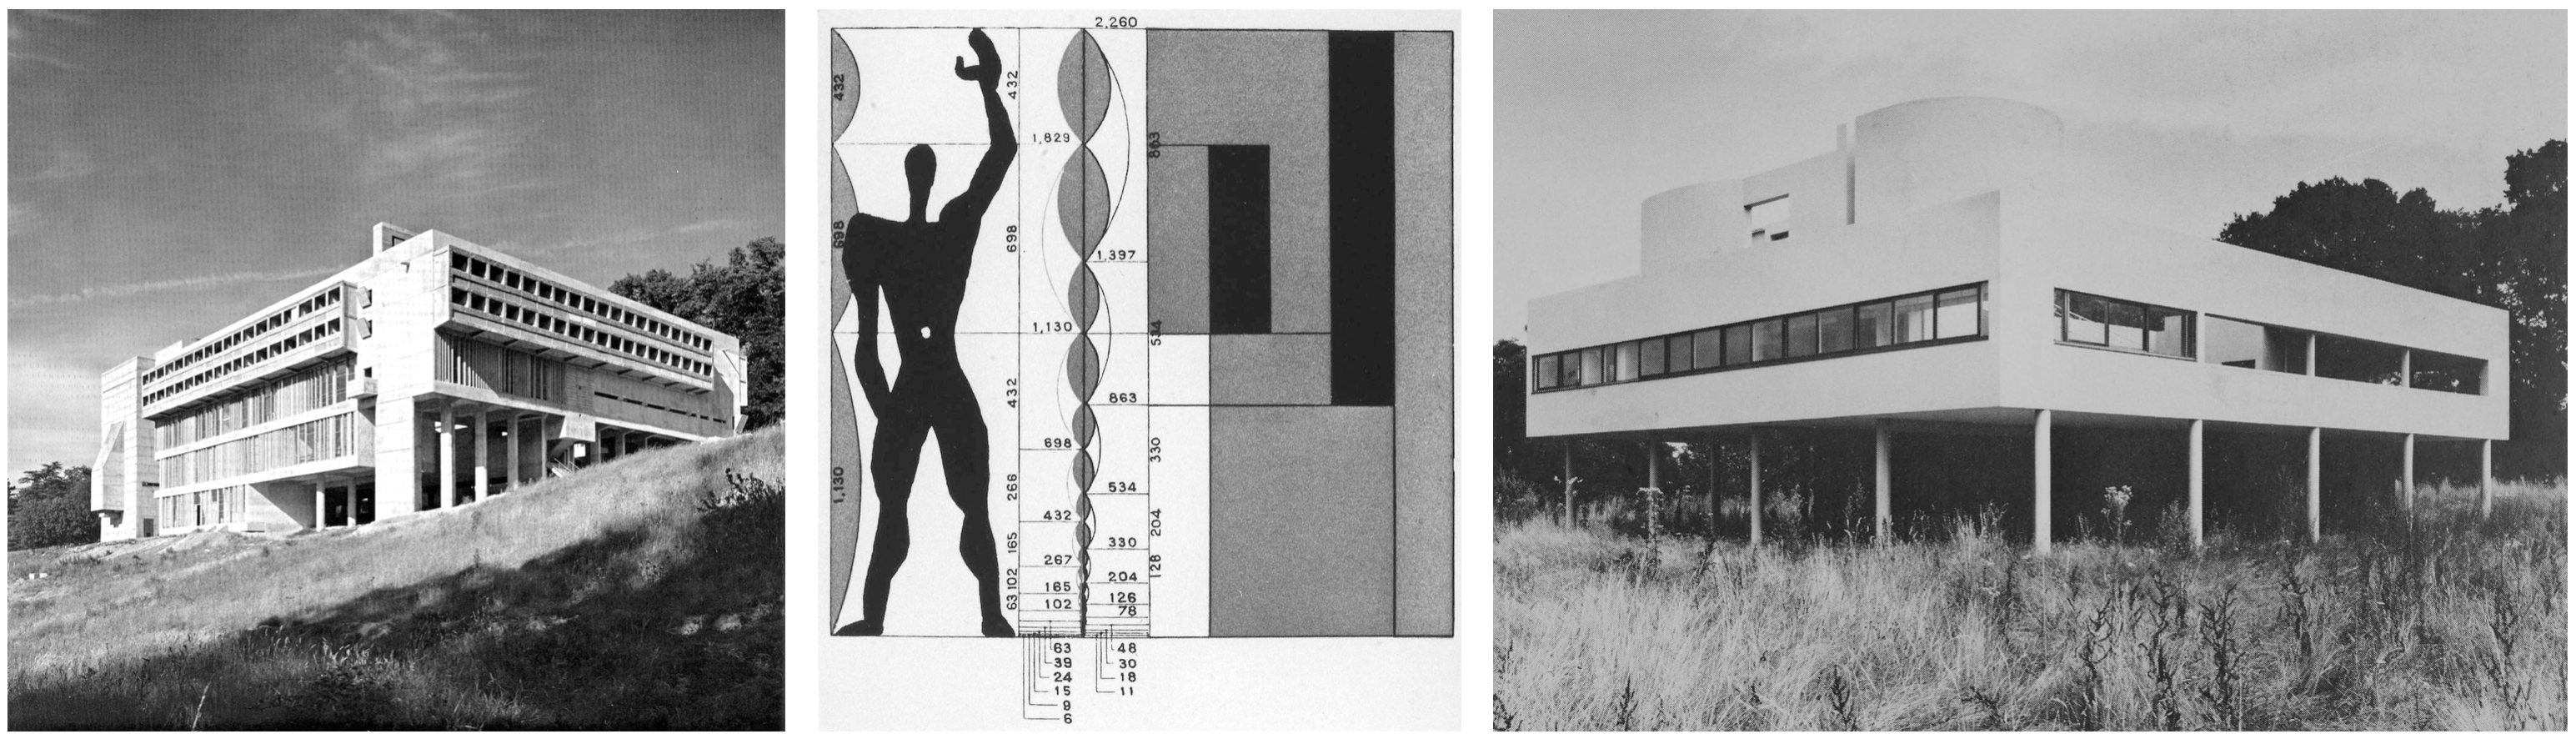
\includegraphics[width=\linewidth]{slideshow}%
  \caption{La Tourette, der Modulor, Villa Savoye}%
  \label{fig:fullfig}%
\end{figure*}

%\begin{fullwidth}
%\small\itshape\lipsum[1]
%\end{fullwidth}


%\footnote{This is a sidenote that was entered
%using the \texttt{\textbackslash footnote} command.}  
%
%\marginnote{This is a
%margin note.  Notice that there isn't a number preceding the note, and
%there is no number in the main text where this note was written.}
%
%\sidenote{The first paragraph of this document includes a citation.}



\section{Literatur}\label{sec:lit}

\begin{fullwidth}

\noindent von Vegesack, Alexander (Hrsg.): \emph{Le Corbusier - The Art of Architecture}, Weil am Rhein 2007.\\

\noindent Le Corbusier: \emph{New World of Space}, New York 1948.\\

\noindent Le Corbusier: \emph{Vers une architecture}, Paris 1923.\\

\noindent Dalrymple, Theodore: \emph{"`Der totalit"are Architekt. Le Corbusiers unheilvoller Einfluss dauert an"'}, in: Merkur, Heft 04, Stuttgart 2010.\\

\noindent Gargiani, Roberto/ Rosellini, Anna: \emph{Le Corbusier. B\'eton Brut und der Unbeschreibliche Raum (1940 -- 1965): Oberfl"achenmaterialien und die Psychophysiologie des Sehens}, M"unchen 2014.\\

\end{fullwidth}
%\nocite{*}
%\bibliography{corbusier}
%\bibliographystyle{plainnat}



\end{document}
